\section{Repr\'esentations informatiques}

	\frame
	{
		\frametitle{Repr\'esentations num\'eriques}
		\begin{itemize}
			\item Repr\'esentation num\'erique : \emph{syst\`eme de num\'eration}.
			\item Syst\`eme de num\'eration connu, le \emph{d\'ecimal}, avec $10$ symboles :
				
			$0$ $1$ $2$ $3$ $4$ $5$ $6$ $7$ $8$ $9$
			\item Soit le nombre 1\textcolor{blue}{9}\textcolor{red}{9} :
			
			\textcolor{blue}{9}$~\neq~$\textcolor{red}{9}
			$\Rightarrow$ valeur d\'epend de la position : \emph{syst\`eme de num\'eration positionnel}.

			\item $0 \rightarrow 1\rightarrow  2 \rightarrow 3 \rightarrow 4 \rightarrow 5 \rightarrow 6 \rightarrow 7 \rightarrow 8 \rightarrow 9\rightarrow ?$ : on \emph{incr\'emente la position suivante} $\rightarrow 10$
			
			$10$ symboles $\Rightarrow$ \emph{base 10} : \emph{syst\`eme de num\'eration positionnel en base 10}.
		\end{itemize}
	}
	
	\frame
	{
		\frametitle{Notion de \emph{base}}
		
		Une repr\'esentation num\'erique doit \^etre adapt\'ee \`a ce qu'elle compte.
		\begin{itemize}
			\item Base $10$ : $10$ doigts.
			\item Autre base connue :  $60$.
			\item \'Electronique (et par extension informatique) :
			\begin{itemize}
				\item base $2$,
				\item ou \emph{binaire},
				\item $1/0$, soit du courant/pas de courant.
			\end{itemize}
			\item Informatique
			\begin{itemize}
				\item base $4$ (Bi-Binaire),
				\item base $8$ (octal),
				\item ou base $16$ (hexad\'ecimal) : 0 1 2 3 4 5 6 7 8 9 A($=10$) B($=11$) C($=12$) D($=13$) E($=14$) F($=15$).
			\end{itemize}
		\end{itemize}
	}
	
	\frame
	{
		\frametitle{G\'en\'eralisation}
		\begin{block}{D\'efinition}
			Soit $x$ un nombre \`a $n$ chiffres dans le syst\`eme de num\'eration positionnel en base $b$.
			
			Alors $x$ s'\'ecrit
			
			$x_{n-1}x_{n-2}\ldots x_1x_0$
			
			et $x=\sum\limits_{i = 0}^{n-1}x_i\cdot b^i$.
		\end{block}
		
		Exemples :
		\begin{description}
			\item $2015_{10} = 2\cdot10^3 + 0\cdot10^2 + 1\cdot10^1+5\cdot10^0$
			\item $199_{10} = 1\cdot2^7 + 1\cdot2^6 + 0\cdot2^5+0\cdot2^4 + 0\cdot2^3 + 1\cdot2^2 + 1\cdot2^1+1\cdot2^0 = 11000111_2$
		\end{description}
	}

\frame
{
	\frametitle{Little ou Big Endian}
	\begin{itemize}
		\item Origines chaotiques de l'informatique.
		\item Diff\'erents ordres de stockage pour les valeurs encod\'ees sur plusieurs octets (1 octet = 8 bits = $2^8$ possibilit\'es = 256 valeurs).
		\begin{itemize}
			\item Little Endian : moins importants en dernier.
			\item Big Endian : plus importants en dernier.
		\end{itemize}
		\item Exemple avec l'entier 2015 :
		\begin{itemize}
			\item Sur 2 octets
			\begin{itemize}
				\item Little Endian : 0x07DF
				\item Big Endian : 0xDF07
			\end{itemize}
			\item Sur 4 octets
			\begin{itemize}
				\item Little Endian : 0x000007DF
				\item Big Endian : 0xDF070000
			\end{itemize}
		\end{itemize}
	\end{itemize}
}

\frame
{
    \frametitle{Le rapport avec DICOM ?}
    \begin{itemize}
        \item Un Data Element contient 4 champs (Tag, Value Representation, Size, Value) dont :
        \begin{description}
            \item[Tag] En h\'exad\'ecimal.
            \item[VR] Le type d'encodage de la valeur.\\
                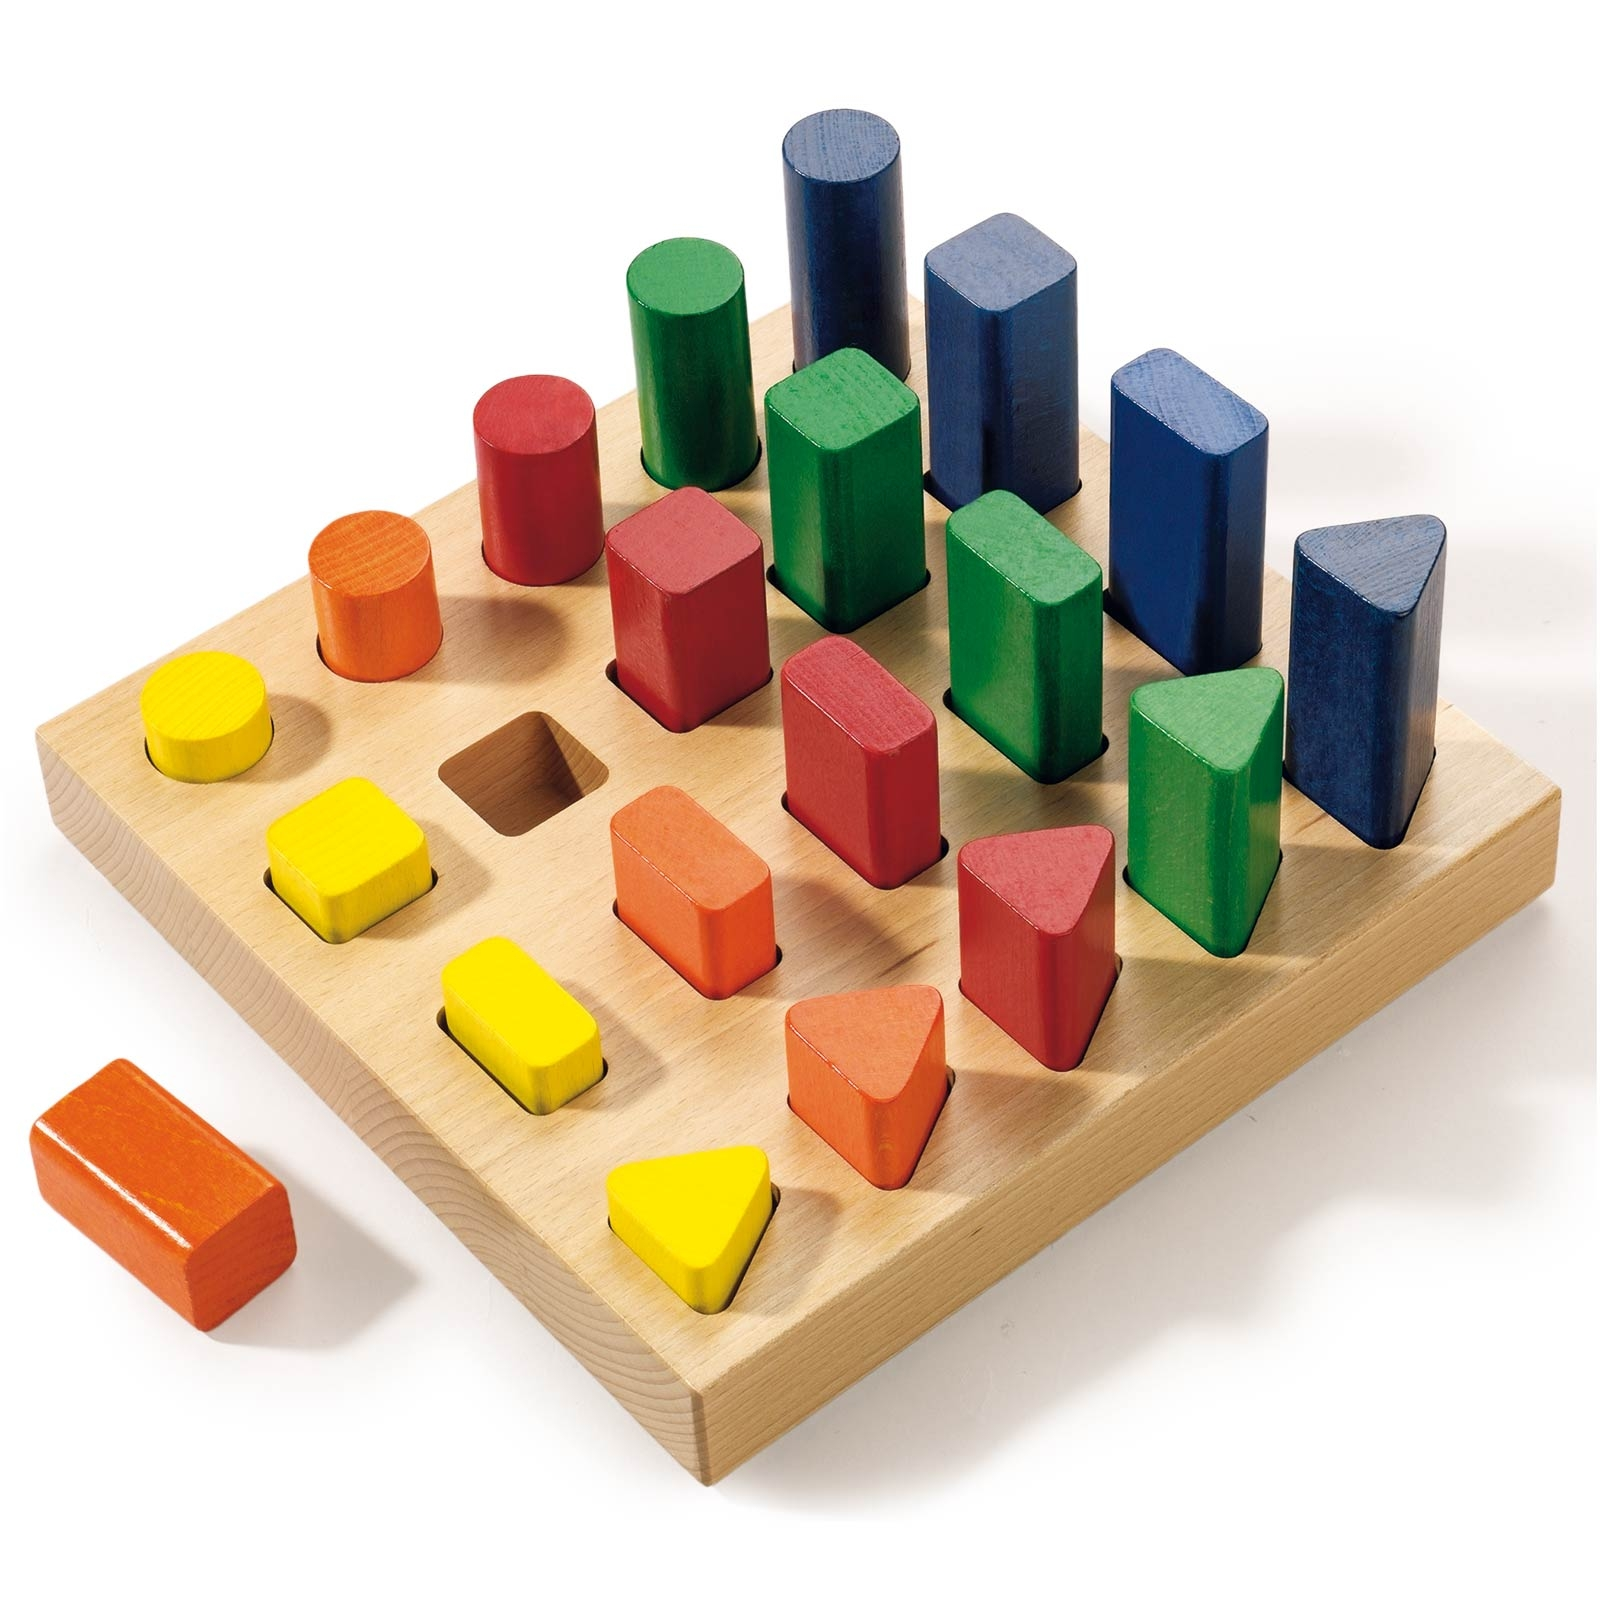
\includegraphics[width=.5\linewidth]{./figures/types.jpg}
        \end{description}
        \item Certains DICOM cod\'es en Little Endian, d'autre en Big Endian. 
    \end{itemize}
}

\frame
{
    \frametitle{Types de VR}
    L'ensemble des VR existants est d\'efini dans la table 6.2-1 \emph{DICOM Value Representation} du standard.

    Quelques exemples :
    \begin{description}
        \item[AS] Age String (e.g. 023Y, 005M, 012D).
        \item[DA] Date, au format YYYYMMDD.
        \item[DT] Date Time, YYYYMMDDHHMMSS.FFFFFF\&{}ZZXX.
        \item[OD] Other Double String (suite de $2^{32}$ octets maximum).
        \item[PN] Person Name (e.g. Doe\^{}John).
        \item[UI] Unique Identifier (UID), 64 caract\`eres maximum (\{0-9,.\}).
    \end{description}
}

